%=== Chapter Three ===
\chapter{Fitting Smooth Arcs to Polygon Regions - Comparative Results}

\section{Introduction}
To understand the advantages of using clothoid pieces to join two poses in a 2D obstacle field, it is informative to compare the output paths with an alternative curve type. One well known option is to use polynomial curves of  degree 3. 

\section{Methodology}
The paths are compared on two simulated environments. One is dimensioned for a small AGV with turning radius 0.5m, as might be used to deliver small items in a flexible manufacturing environment. The unexpected obstacle completely blocks the path to the right as in Figure \ref{fig:env1}. The second could represent a fork lift type AGV with a larger turning radius of 2m, which is collecting standard size (1m x1.2m) pallets from a storage area. See Figure \ref{fig:env1}. The pallets are placed by human drivers, and a reliable system fo detecting their position and orientation is assumed to be in place. The AGV must manoeuvrer to the pose of a target pallet, without colliding with the others. Lower curvature and sharpness allow the AGV to traverse the path faster without compromising load stability.

\section{Algorithm}
Both methods decompose the problem into topology followed by curve fitting. The topology problem is a posed as a directed graph with weighted edges. There is a node for every intersection of the boundary between two regions. Nodes within the same region are fully connected. The weight of each edge corresponds to the euclidean distance between the two nodes. The A* Algorithm is used to search for the set of edges which give the minimum sum of weights between any start and end pose.

The sequence of edges is then used to populate the matrix $\bm{H} ^{(R \times P)} \in [0,1]$. This is a binary matrix containing $R$ columns, one for each of the $R$ polygonal regions which comprise the accessible space. Each row corresponds to one of the $P$ path pieces and contains a single non-zero element indicating the region to which is assigned. A path piece may be present in more than one region as the regions may be overlapping, but it must always remain completely inside its assigned region.

\subsection{Polynomial Method}
The problem specification calls for a path which changes smoothly in x, y, heading and curvature. This should start at a specified $x_s, y_s, \psi_s$ with zero curvature and end at $x_g, y_g, \psi_g$ with zero curvature.

\begin{equation}
\begin{array}{c}
x(t) = a + bt + ct^2 + dt^3 \\
y(t) = e + ft + gt^2 + ht^3 \\
\end{array}
\label{eq:spline}
\end{equation}

There is a unique solution for a cubic spline of with fixed (x, y, heading) at the start and goal, passing through fixed $x, y$ positions numbering $n$. A cubic spline defined by Equation \ref{eq:spline} has eight free parameters per segment. To give a unique solution, eight constraints are must be found for each segment. Passing through the $n$ waypoints at the end of each segment gives two, one for the $x$ coordinate and one for $y$. Enforcing continuity of position between the end of each segment and the next leads to two more. Four more can be determined from continuity in the first and second derivative of position for a total of eight. 

However, only four constraints are needed at the start and end of the spline. Fixing the final position and heading, the acceleration must be left free. Stacking the parameters into a vector 
\begin{equation}
\bm{p}_i = [a_i, b_i, c_i, d_i, e_i, f_i, g_i]^T
\end{equation} 
and 
\begin{equation}
\bm{p} = [\bm{p}_1,\cdots,\bm{p}_i, \cdots, \bm{p}_{n-1}]^T
\end{equation} 
leads to the system of linear equations is given in Equation \ref{eq:assembled}. 

\begin{equation}
[\bm{A}|\bm{b}_{x}] = \left[\begin{array}{cccccc|c}
\bm{A}_{0} & & & & \cdots & 0 & \bm{b}_{x0}\\
\bm{0} & \bm{A}_{1} & & & \cdots & 0 & \bm{b}_{x1}\\
\vdots & 	& \ddots &	& 	& \vdots	& \vdots \\
0 & & \cdots & \bm{A}_{i} &  \cdots & 0 & \bm{b}_{xi}\\
\vdots & 	& 	&	& \ddots  &		& \vdots \\
0 & \cdots &  &  & &  \bm{A}_{n} 			& \bm{b}_{xn}\\
\end{array}\right] 
\label{eq:assembled}
\end{equation}

Where
\begin{equation}
[\bm{A}_{0}|\bm{b}_{x0}] = \left[ \begin{array}{cccc|c}
1 & 0 & 0 & 0 & x_0\\
0 & 1 & 0 & 0 & \cos{\phi_0}\\
\end{array} \right] 
\label{eq:submatrix_0}
\end{equation}

\begin{equation}
[\bm{A}_{i}|\bm{b}_{xi}] = \left[\begin{array}{cccccccc|c}
1 & 1 & 1 & 1 & 0 & 0 & 0 & 0 & x_{i}\\
1 & 1 & 1 & 1 & -1 & 0 & 0 & 0 & 0\\
1 & 1 & 2 & 3 & 0 & -1 & 0 & 0 & 0\\
0 & 0 & 2 & 6 & 0 & 0 & -2 & 0 & 0
\end{array}\right]
\label{eq:submatrix_i}
\end{equation}

\begin{equation}
[\bm{A}_{n}|\bm{b}_{xn}] = \left[\begin{array}{cccccccc|c}
0 & 0 & 0 & 0 & 1 & 1 & 1 & 1 &x_n\\
0 & 1 & 0 & 0 & 0 & 1 & 2 & 3 & \cos{\psi_n}\\
\end{array}\right] 
\label{eq:submatrix_n}
\end{equation}

The $\bm{p}_x$ parameters to fit a set of $n$ waypoints can be found by computing $\bm{p}_x = \bm{A}^{-1}\bm{b}_x$. The $\bm{p}_y$ parameters can be found almost identically, by computing $\bm{p}_y=\bm{A}^{-1}\bm{b}_y$. Constraint vector $\bm{b}_y$ is instead constructed using the $y$ coordinates of the waypoints in $b_i$ and the $\sin$ of the start and end heading in $\bm{b}_{y0}$ and $\bm{b}_{yn}$.

\section{Optimisation}
The point to point solution through the region intersection points is quite a good solution. Continuous in $\dot{X}$ and $\ddot{X}$, it reaches the goal position and heading. It is excessively constrained by the requirement to meet the intermediate waypoints.
Using the optimisation in Equation \ref{eq:full_opt}  
\begin{equation}
\begin{array}{c}
\min \sum_{j=1}^N ||\frac{dP_j^3(t)}{dt^3}||^2 \\
\textrm{subject to} \\
P_j(1) = P_{j+1}(0) \\
\dot{P_j}(1) = \dot{P_j}(0) \\
\ddot{P_j}(1) = \ddot{P_j}(0) \\
P_1(0) = X_S \\ 
P_N(1) = X_G \\
\dot{P_1}(0) = \dot{X_S} \\
\dot{P_N}(1) = \dot{X_G} \\ 
\textrm{also subject to} \\
\bm{H}_{j,r} \Rightarrow X_r^{min} \leq P_j(t) \leq X_r^{max} 
\end{array}
\label{eq:full_opt}
\end{equation}

The implementation of the region constraint in Equation \ref{eq:full_opt} must ensure the entire arc remains inside the assigned region according to $\bm{H}$. For piecewise linear arcs this can be done by checking the containment of the start $P_0(0)$ and end $P_N(1)$. Got cubic splines it is more challenging. Deits and Tedrake \ref{Deits2015} describe an approach based on Sum of Squares, where a small Semidefinite Program is solved in the parameters of $P_j$, to avoid sampling at different $t$ values, which can lead to the path cutting corners and even passing through thin obstacles.

First we notice that the constraints on one segment from its axis aligned containing region described by $x_min, x_max, y_min, y_max$ can be written as vector inequality
\begin{equation}
 q(t) = \left[\begin{array}{c}
 x_{max} - a - bt - ct^2 - dt^3 \\ 
 a + bt+ ct^2 + dt^3 - x_{min} \\
 y_{max} - e - ft - gt^2 - ht^3 \\ 
 e + ft+ gt^2 + ht^3 - y_{min} \\
 \end{array}\right] \geq \bm{0} \forall t \in [0,1]
 \label{eq:qt}
 \end{equation}
. The condition in Equation \ref{eq:qt} can only hold if and only if it can be rewritten in the form
\begin{equation}
t\sigma_1(t) + (1-t)\sigma_2(t)
\end{equation}
. This leads to 
\begin{equation}
\sigma_1(t) = \left[\begin{array}{c}
	x_{max} - a- b- ct- dt^2 \\
	a + b+ ct+ dt^2 - x_{min} \\
	y_{max} - e - f - gt - ht^2 \\
	e + f+ gt+ ht^2 +-y_{min} \\
	\end{array}\right]
\end{equation}
and 
\begin{equation}
\sigma_2 = \left[\begin{array}{c}
x_{max} -a \\
a - x_{min} \\
y_{max} - e \\
e - y_{min} \\
\end{array}\right]
\end{equation}. 
The standard Sum of Squares approach calls for collecting the parameters of $\sigma(t)$ by the order of $t$. Matching coefficients against
\begin{equation}
\sigma_i = \beta_1 + \beta_2 t + \beta_3 t^2
\end{equation}, gives
\begin{equation}
\beta_1 = \left[\begin{array}{c}
x_{max} - a - b \\
a + b - x_{min} \\
y_{max} - e - f \\
e + f + y_{min} \\
x_{max} - a \\
a - x_{min} \\
y_{max} - e \\
e + y_{min} \\
\end{array}\right]
\end{equation}
and
\begin{equation}
\beta_2 = \left[\begin{array}{c}
-c \\
+c  \\
-c \\
+c \\
0\\
0 \\
0 \\
0 \\
\end{array}\right]
\end{equation}
and
\begin{equation}
\beta_3 = \left[\begin{array}{c}
-d \\
+d  \\
-d \\
+d \\
0\\
0 \\
0 \\
0 \\
\end{array}\right]
\end{equation}
. Where the parameters for $\sigma_2$ have been stacked after those from $\sigma_1$. 

In order for $\sigma_i$ to be a sum of squares, there are the following conditions on $\beta_1$, $\beta_2$, $\beta_3$:
\begin{equation}
\begin{array}{c}
4\beta_1\beta_3 - \beta_2^2 \geq 0
\beta_1, \beta_3 \geq 0
\end{array}
\end{equation}

 In the simple case where the regions are axis aligned, this immediately creates a problem as the first two equations have $\beta_3 = d$ and $\beta_3 = -d$. The only value of $d$ which will satisfy the sum of squares condition is zero. However the initial guess which joins the corner points, satisfies the region occupancy constraints with a non-zero $d$. 
 
 For this reason the constraints are enforced using 50 samples for each path piece. This leads to a small degree of corner cutting which must be included in the safety factor used on the vehicle body width used to inflate the obstacle. It also results in a large number of constraints as there are four for each sample. For this to be possible we must use a fixed spatial sampling length rather than a fixed number of samples per piece as path pieces can vary in length substantially which makes the degree of corner cutting variable.
 



\subsection{Clothoid Method}
Initialization with parameters which meet the continuity and obstacle constraints with clothoid pairs proved to be a challenging task. This is expected to improve the convergence time. To generate a set of parameters to meet continuity constraints for initialization of the region method is very similar to the interpolation problem addressed by Bertolazzi et al (2018) \cite{Bertolazzi2018}. The main difference is that the intermediate waypoint headings are free variables in the initialization, unlike in interpolation.

If the waypoint headings are fixed, and curvature at them to zero, the clothoid interpolation problem can be solved for each segment independently, as described by \cite{Gim2017a}. Different point to point methods could be used such as the bisection method \cite{Gim2017b}, geometry \cite{Vazquez-Mendez2016} and minimax sharpness \cite{Henrie2007}. Lacking a natural heading, a heuristic based on the maximum squared sum of $a^2 + b^2$ and requiring $a>0$ and $b<0$ where $a$ is the distance to the intersection point from $P_1$ and $b$ is the distance from $P_2$. The different sign is important for the direction of travel, to put the intersection in front of the first pose and behind the second.

The multiple shooting clothoid method uses additional parameters for the start pose of every segment. If this was initialized to zero, interior-point method reached convergence in about 70 seconds in environment 2. None of the more involved methods improved on this so we used the simple approach for further testing.  

\section{Convergence dependence on $b$}
\begin{figure}
	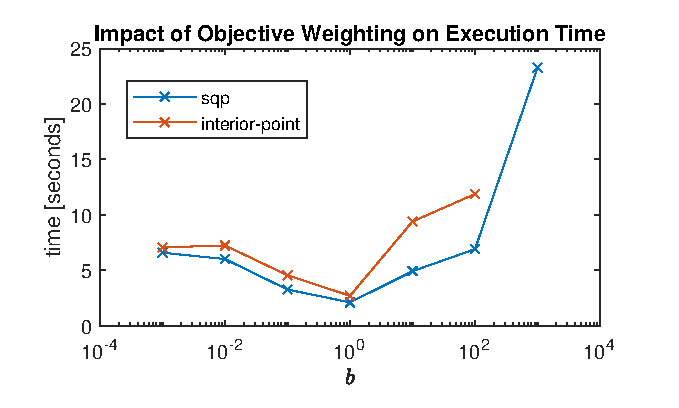
\includegraphics[width=0.5\linewidth]{w_convergence_time_SMALL}
	\label{fig:w_convergence}
	\caption{Convergence time variation with weighting on item fetch environment}
\end{figure}

In environment 1 both large and small values of $w$ led to poor convergence. One possible explanation is numerical conditioning being damaged by the weighting. A large $w$ results in a solution with small $\alpha$, while the length remains on the same order. Some matrix operations may return inaccurate results with different magnitude parameters.
\begin{table}
\begin{center}
	\begin{tabular}{ |c|c|c|c|c| }
		\hline
		 $b$ & $1\times10^{-3}$&  1 & 100 & 1000* \\ 
		 \hline
		 fevals &7929 & 10873 & 11986& 200,000* \\  
		 execution time (s)& 55 & 72 & 80 & 1345* \\
		 path length (m) & 7.071 & 11.694 & 36.038 & 5.695*\\
		 \hline  
	\end{tabular} \\
		 *Convergence Failure
\end{center}
\label{tab:b_dependence}
\caption{Convergence for different $b$ values for the multiple shooting approach, in pallet environment} 
\end{table}
To test the hypothesis that only method using dense matrices such as sqp would be affected, the effect on the interior point method (which does not depend on dense matrix operations) is reported in Table \ref{tab:b_dependence}. This shows that changing the weighting damages convergence significantly to the extent that no valid result is found even after 200000 function evaluations. There were no warnings printed by fmincon during this run. The value of feasibilty was positive of the order 1e-6 and decreasing very slowly, while the objective function was large of the order 1e6 and also decreasing very slowly (relative to its magnitude).

Contrary to expectation, reducing $b$ to emphasize the path length reduced the number of iterations to convergence. Table  \ref{tab:b_dependence} shows an inverse relationship between $b$ and the number of iterations. Sufficiently large $b$ makes the problem more difficult to solve as the path segments deflect further, making a linear approximation worse. This effect is indirect because the constraints use the precise nonlinear dynamics and the interior-point method does not solve a series of linear approximations to the constraints like sqp. Interior point should always converge if given an initial guess in the feasible reason, unless the problem is non-convex. The initial graph step intended to remove non-convex elements of the problem may lead to suboptimal paths as the segments deviate from straight lines. But this does not explain the increasing number of iterations. 

Curvature is more weakly linked to the parameters than the total length. The curvature objective is the squared sum of $2r$ parameters while the length objective is the squared sum of $4r$ parameters. Both of them leave numerous parameters to be coupled through the constraints as in total there are $9r$ parameters for the multiple shooting formulation. 

\section{Generating a Convex Region Representation from LIDAR Data}
A widely used representation for a 2D obstacle field is an occupancy grid \cite{Thrun1996}. Also see Probabilistic Robotics textbook \cite{thrun2005probabilistic} for details on creating a map from sensor data. Each cell represents an area of the floor, with a number $p\in[0,1]$ indicating the probability it contains an obstacle. Thresholding can be used to create a binary map of occupied and unoccupied cells. In order to connect adjacent unoccupied cells to form regions numerous approaches from image processing are available. A method suitable for simple environments is vertical cell decomposition \cite{LaValle2006c}. This begins with piecewise linear polygons, which can be created by connecting the cell corners of a binary occupancy grid.


\section{Test Environment}
The test environment was created for an automated fork lift AGV research platform which is taken to be representative \cite{Baird2018}. The obstacles are based on $(1.0 \times 1.2)$m pallets which are commonly used in the UK and Netherlands \cite{Raballand2005}. The datasheet for the manually operated vehicle on which the AGV is based, a Hyster E30-40HSD gives the dimensions in Table \ref{tab:dimensions}. The dimensions are drawn on a plan of the vehicle in Figure \ref{fig:fork_dims_circ}.

\begin{figure}
	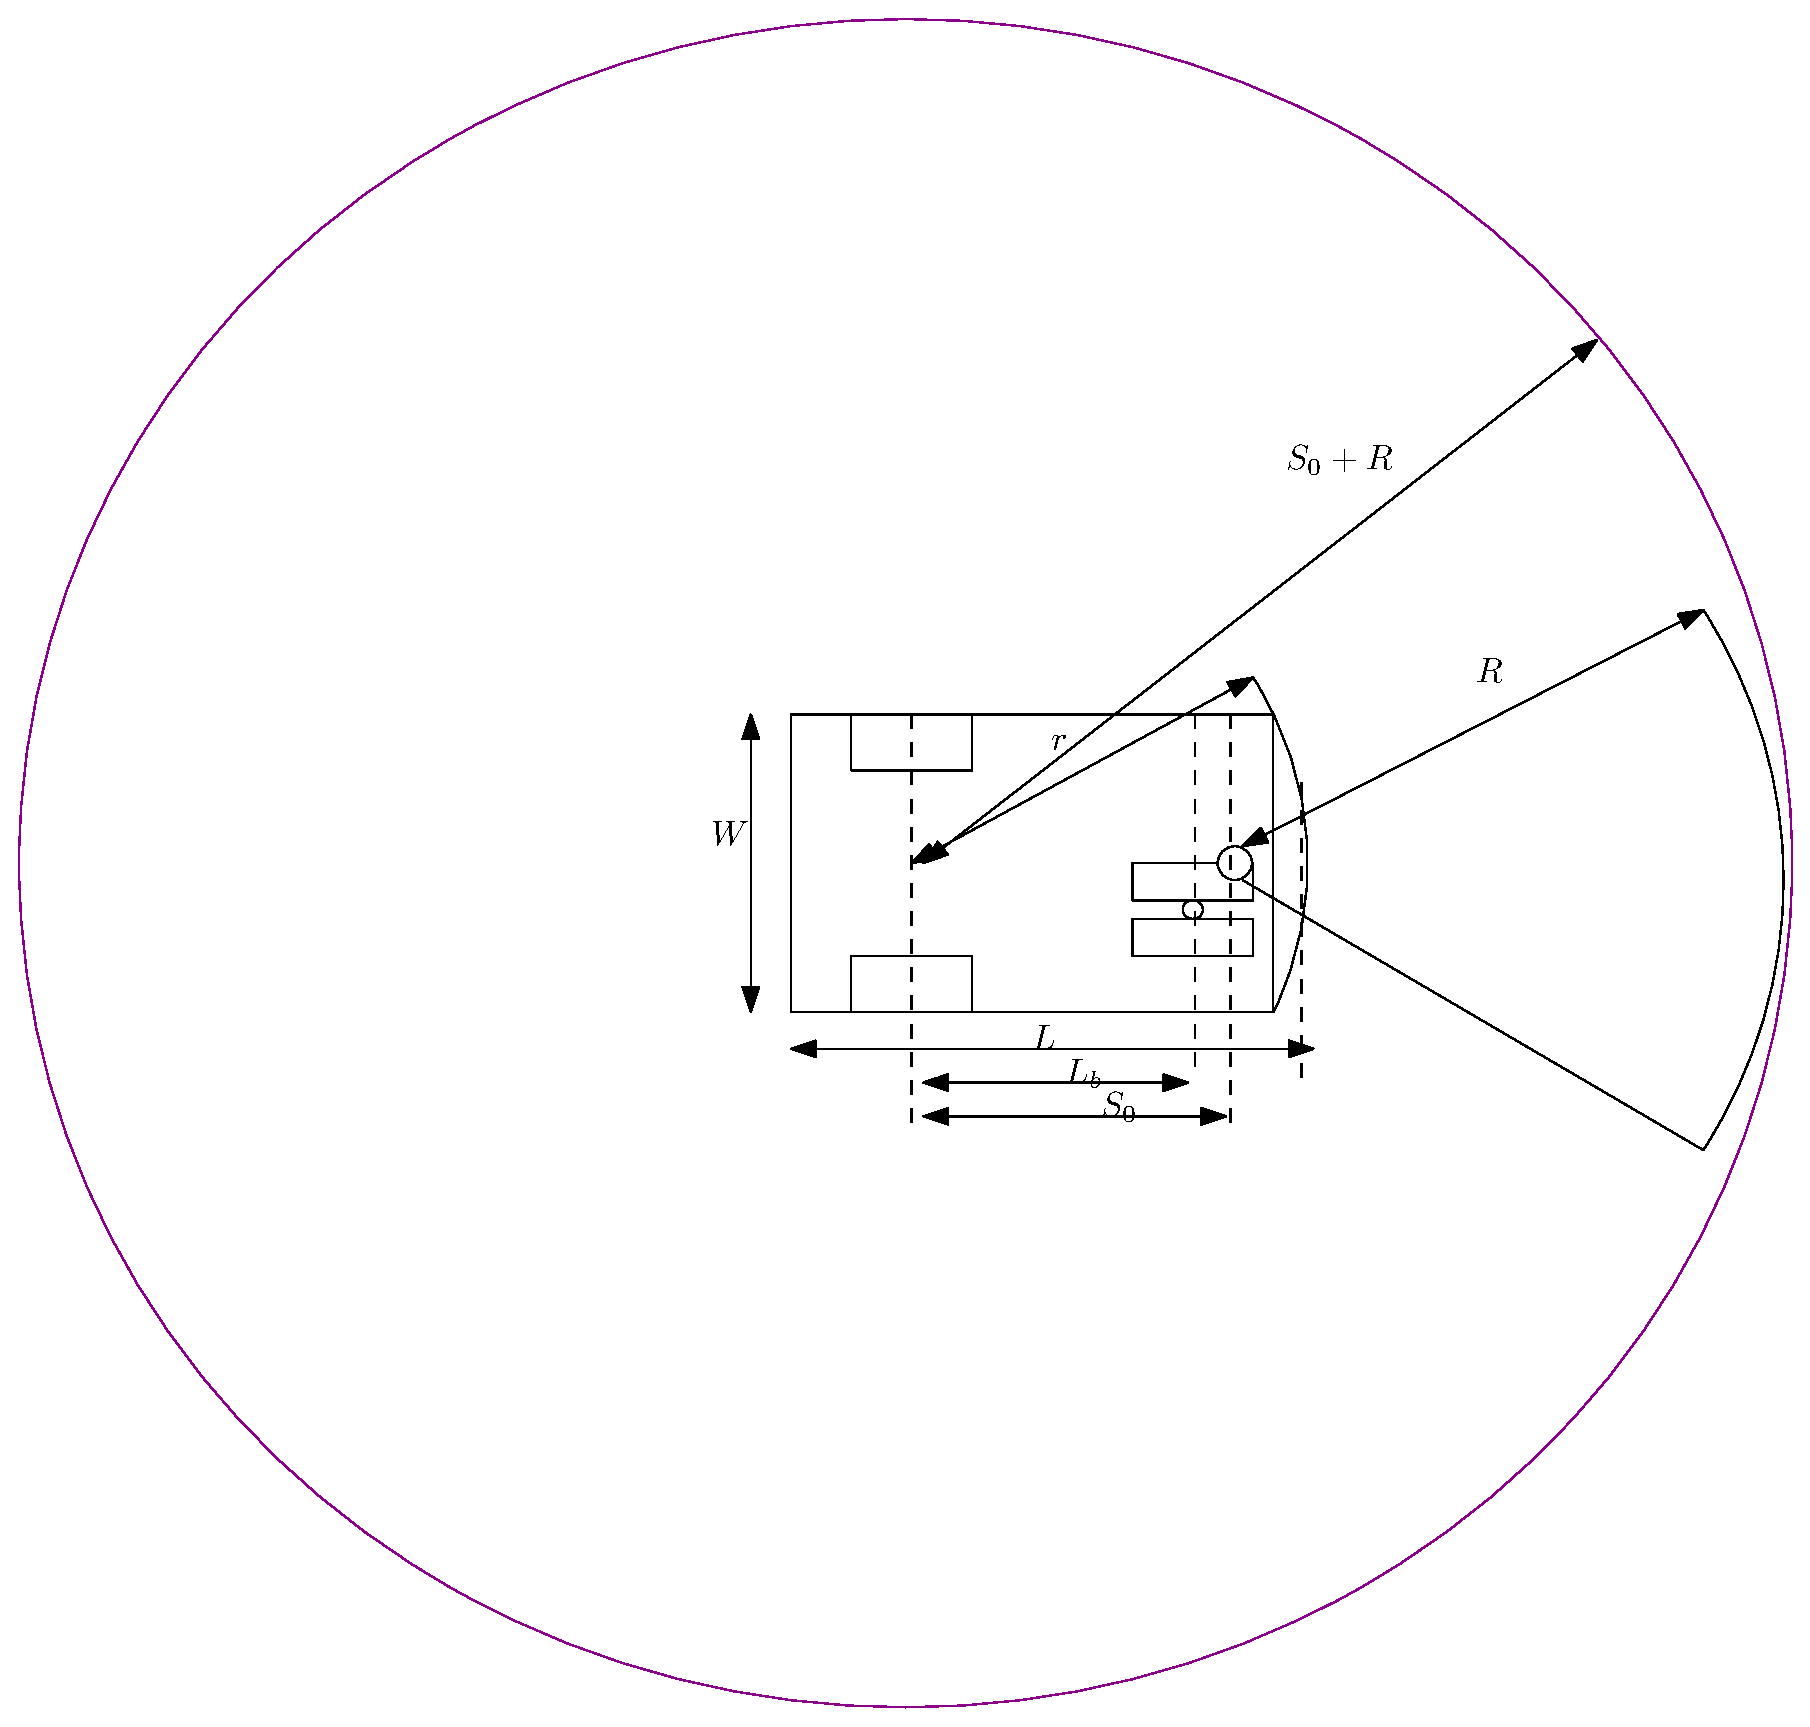
\includegraphics[width=0.5\linewidth]{fork_dims_circ}
	\label{fig:fork_dims_circ}
	\caption{Dimensions used to expand the obstacles}
\end{figure}
\begin{table}
	\begin{center}
		\begin{tabular}{ |c|c| }
			\hline
			Parameter & Dimension (mm) \\
			\hline
			$W$ & 1067 \\
			$L$ & 1583 \\
			$r$ & 1289 \\
			$L_s$ & 1001 \\
			$S_0$* & 1200 \\
			$R$* & 1300 \\
			\hline  
		\end{tabular} 
	\end{center}
	\label{tab:dimensions}
	\caption{Dimensions from datasheet. *Stopping distance $R$ based on top speed 3.22m/s and hypothetical braking deceleration of 4m/s$^2$} 
\end{table}
The datasheet gives the maximum speed as 7.2 miles per hour (3.22m/s). Traction is provided by dual 4.8kw motors. The unloaded weight of the vehicle is 3059kg and the battery 1043kg for a total of 4201kg.  

For correct operation it is important to consider the exclusion zone of the safety rated range sensor fitted to the front of the vehicle. If an obstacle breaches the exclusion zone the AGV must perform an emergence stop, or in some cases slow down significantly. To avoid slowing down the path planning must account for not only the shape of the vehicle but also the shape of this zone. Often this is a cuboid slightly wider than the vehicle, sufficiently long that the AGV can come to a complete stop from full speed before the front makes contact with a static obstacle. More details are available in the NIST Safety Standards \cite{Bostelmann2013}. To avoid 

In the two simulated environments the obstacle field is represented in 2D. The bounding circle dimension is strongly influenced by the stopping distance $R$. 
Starting from the constant acceleration equation
$v^2 = u^2  + 2as$ and setting $v=0$ gives the stopping distance $s = \frac{u^2}{-2a}$. 
\begin{figure}
	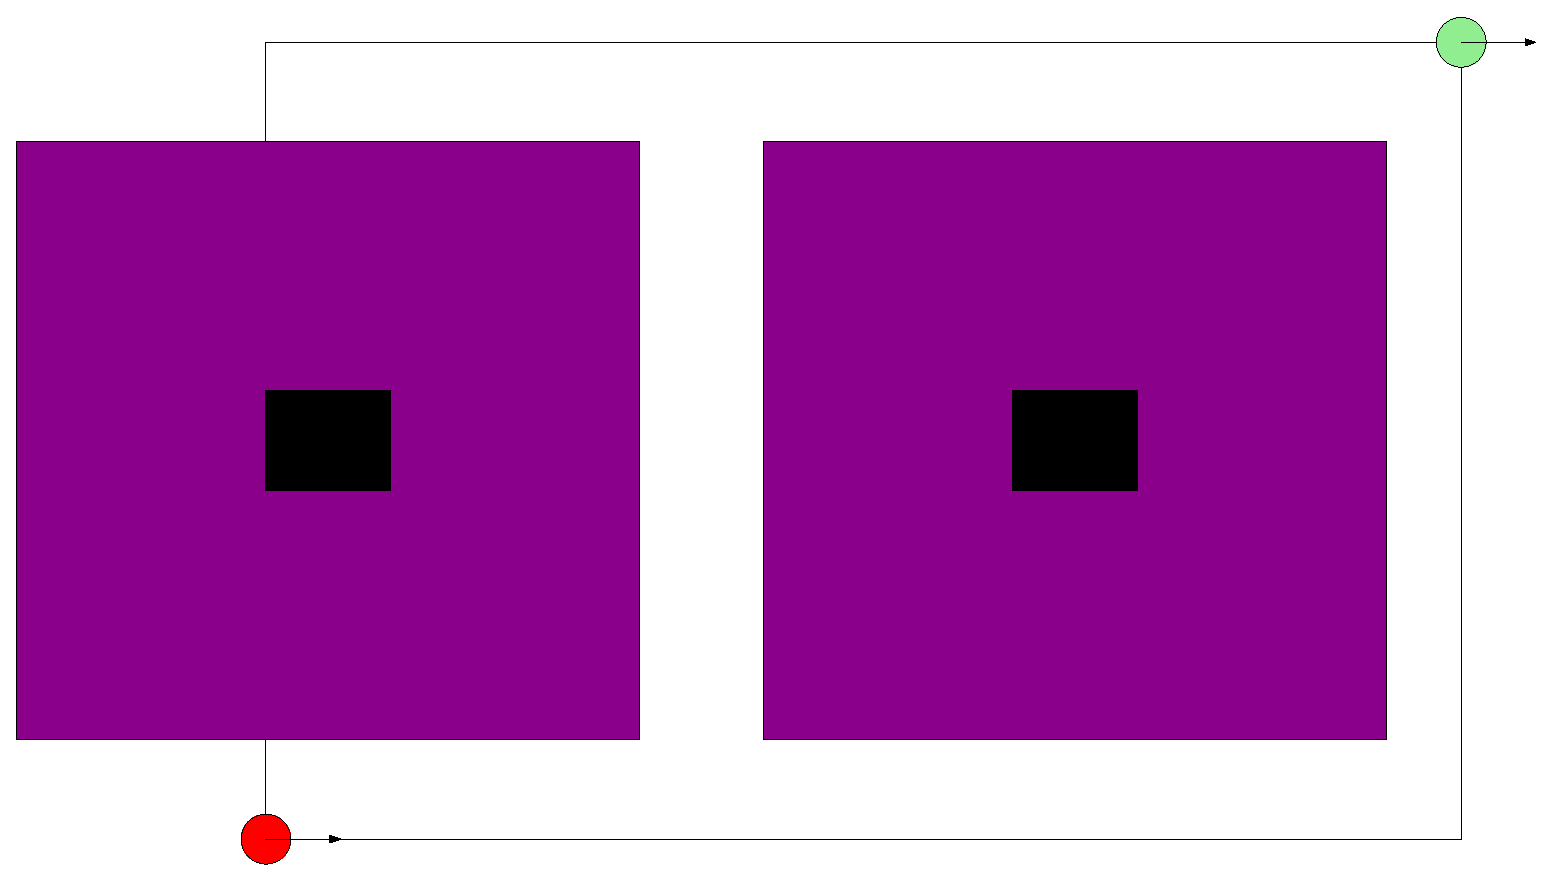
\includegraphics[width=0.5\linewidth]{pallet_env_expand_2point5}
	\label{fig:pallet_env}
	\caption{Pallet environment. Obstacles are black with expansion by the vehicle disk shown in purple.}
\end{figure}

Expanding the environment with a disc the size of the largest dimension of the vehicle is a gross approximation, which will lead to over cautious paths. It would be better to represent the obstacles in (2 + 1) dimensions, and plan in ($x, y, \psi$). Obstacles can then be expanded based on the current heading of the path as described in \cite{Deits2015b} who use a sum of squares approach to find (2+1)D convex polygons. 